\chapter{Introduction}
\section{Energy storage}
\begin{figure}
\centering
\begin{subfigure}{\linewidth}
  \centering
  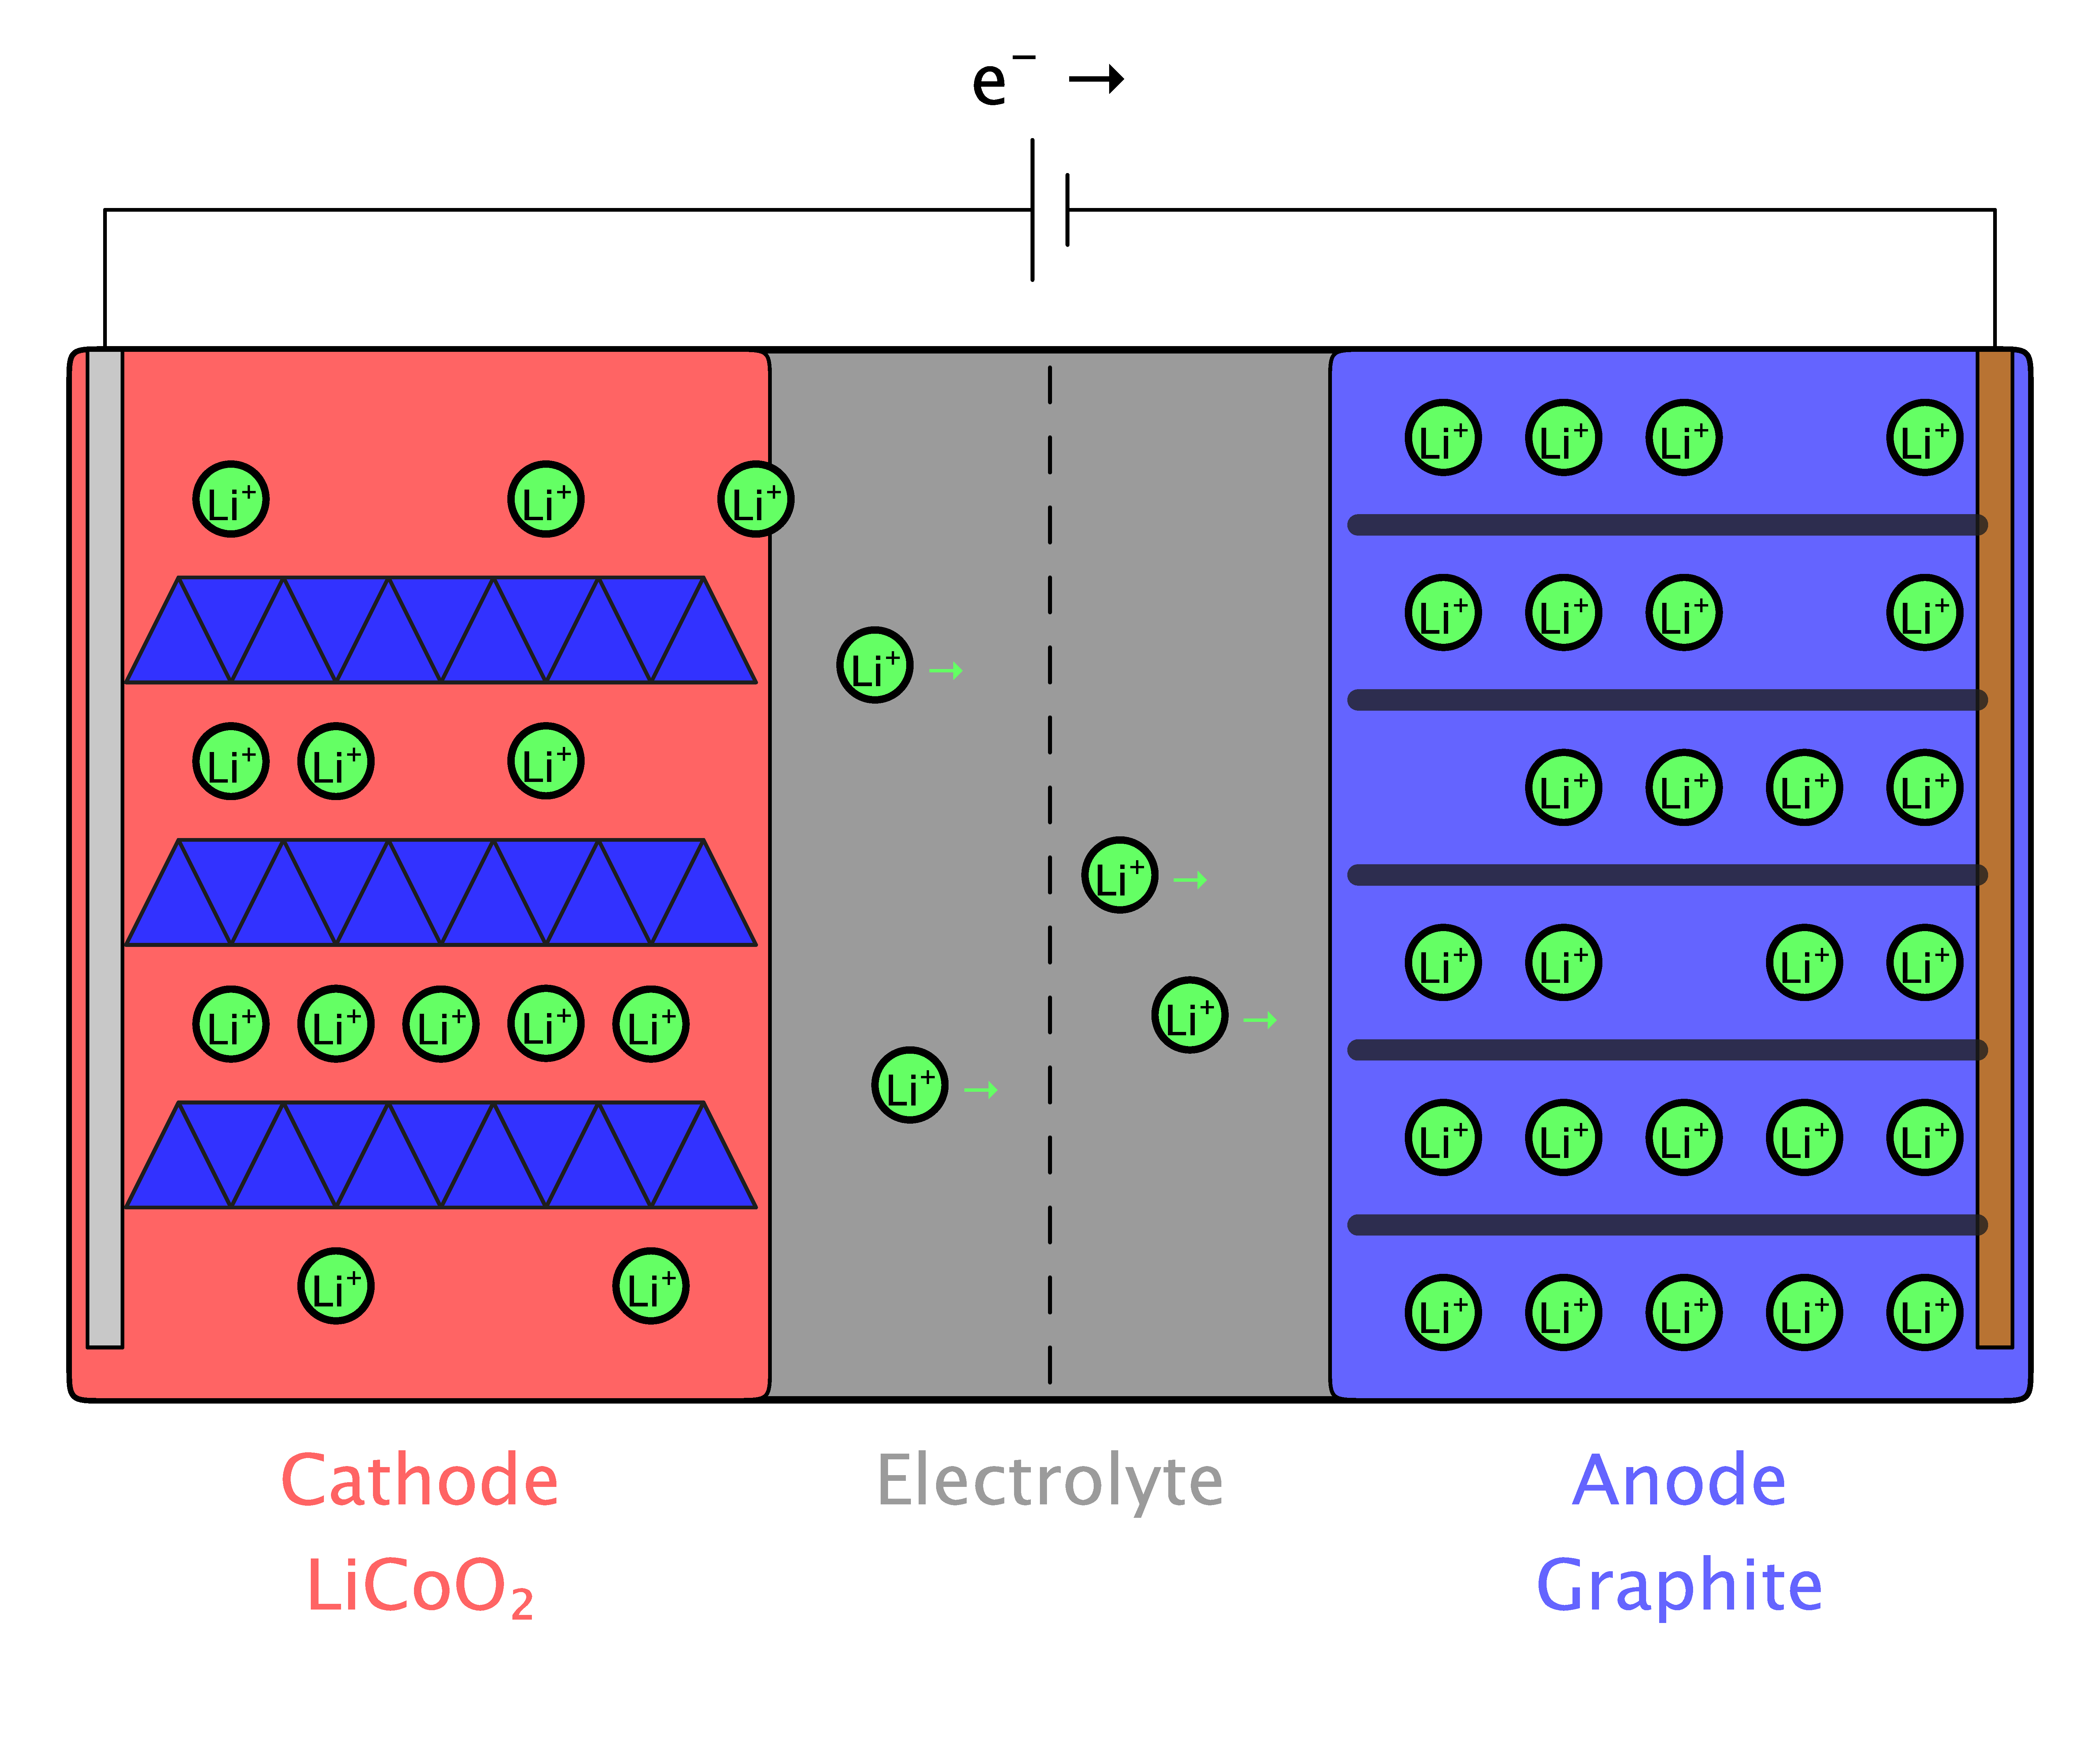
\includegraphics[width=0.7\linewidth]{figures/batteryCharge/batteryCharge}
  \caption{Charging}
  \label{fig:GoodenoughCharging}
\end{subfigure}

\begin{subfigure}{\linewidth}
  \centering
  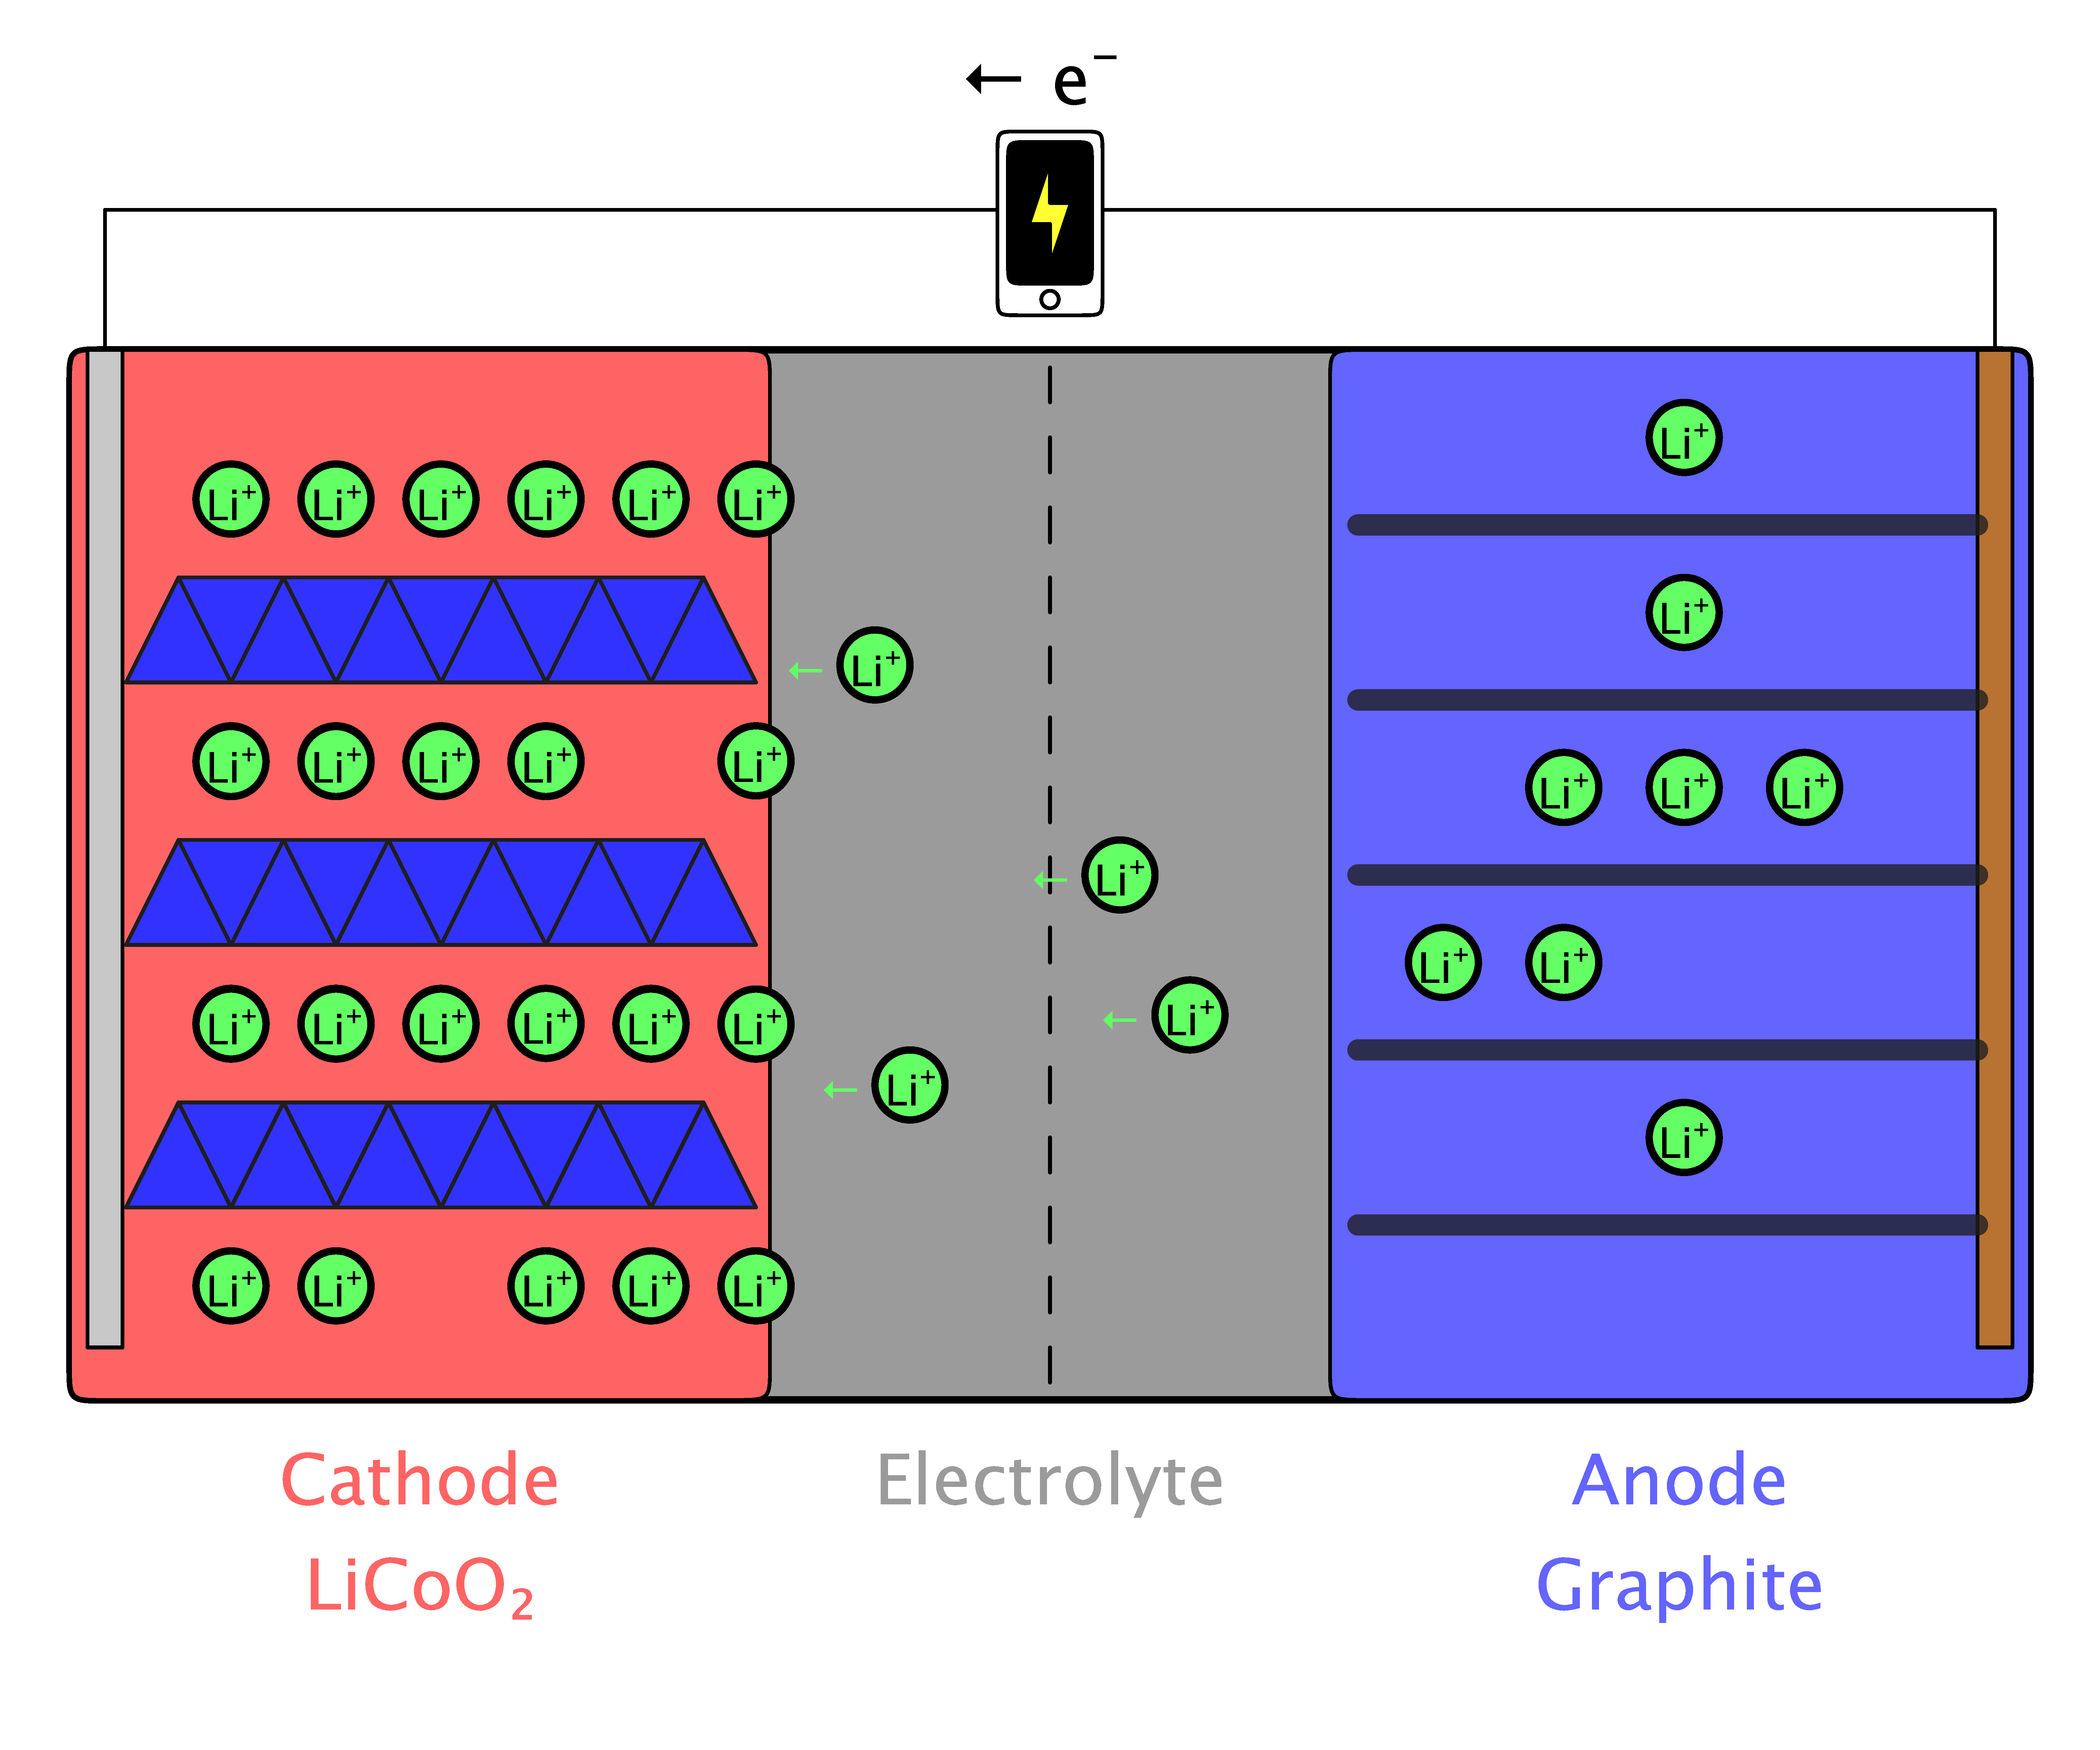
\includegraphics[width=0.7\linewidth]{figures/batteryDischarge/batteryDischarge}
  \caption{Discharging}
  \label{fig:GoodenoughDischarging}
\end{subfigure}
\caption[Li-ion battery schematic]{A schematic of a common Li-ion battery. During charging (a), electrons are driven to the anode by an external potential. \ce{Li+} ions move from the cathode to the anode to charge balance. During discharge (b), \ce{Li+} ions are driven to the cathode by a difference in chemical potential. The electrodes are electrically isolated by the separator, and are forced to instead travel via an external circuit and provide work.} 
\label{fig:Goodenough}
\end{figure}
